\documentclass{scrbook}
\usepackage{phd}
\usepackage{luacode}

\begin{filecontents*}{test.json}
{
"recipe": {
    "title":"First recipe",
    "source":"My first cookbook",
    "carbs":"1 oz",
    "fat":"1 oz",
    "protein":"1 oz",
    "cal":"100 kcal",
    "ingredients": [
        {"item":"Eggs"},
        {"item":"Oil"},
        {"item":"Nuts"}
    ],
    "cooking": [
        {"step":"Mix eggs and oil"},
        {"step":"Add nuts"}
    ]
},

"cake": {
    "title":"First recipe",
    "source":"My first cookbook",
    "carbs":"1 oz",
    "fat":"1 oz",
    "protein":"1 oz",
    "cal":"100 kcal",
    "ingredients": [
        {"item":"Eggs"},
        {"item":"Oil"},
        {"item":"Nuts"}
    ],
    "cooking": [
        {"step":"Mix eggs and oil"},
        {"step":"Add nuts"}
    ]
}
}
\end{filecontents*}

\begin{document}

 
\pan
\begin{luacode}
--  We use the lualibs built-in modules
--  this loads all the modules including a json converter
--

local M = M or {}

require("lualibs.lua")


-- @json file
function getjsonfile (file)
    local f, s
	  f = io.open(file, 'r')
        s = f:read('*a')
        f.close()
        return s
 end

local s =  utilities.json.tolua(getjsonfile('test.json'))


local rep, write = string.rep, tex.print

function M.inspect (tab, offset)
   local openbracket, closebracket, par = "\\{", "\\mbox{..}\\}", "\\par"
   
    offset = offset or ""
    for k, v in pairs (tab) do
        local newoffset = offset .. "\\mbox{~~}"
        if type(v) == "table" then
           write(offset .. k .. " = " .. openbracket .. par)
           M.inspect(v, newoffset)
           write(offset .. closebracket .. par)
        else
         if k~="data" then write(offset..k.." =  ".. tostring(v), "\\par") 
           else
                 write(offset.."k = char data ")
           end
       end
    end
end

tex.print(M.inspect(s))

tex.print('\\ttfamily',table.serialize(s))
tex.print('\\par')

print = tex.print


table.print(s)

 inspect(utilities.templates.replace("test %one% test", { one = "%two%", two = "two" }))

tex.print(s.cake.fat  )
 \end{luacode} 
 
\AddToShipoutPicture{%
 \AtTextUpperLeft{%
    \put(500pt,0pt){%
    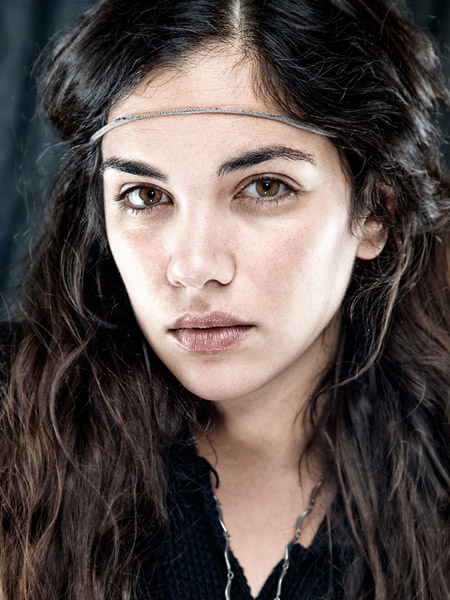
\includegraphics[width=1cm]{./images/amato.jpg}}}
}
 
 \end{document}
